\documentclass[aspectratio=169, 14pt]{beamer}
\usepackage[utf8]{inputenc}
\usepackage{xeCJK}
\usepackage{graphicx}
\usepackage{transparent}
\usepackage[ruled, lined, linesnumbered, commentsnumbered]{algorithm2e}
\usepackage{pgfplots}
\usepackage{tikz}
\usetikzlibrary{matrix,backgrounds}
\usetikzlibrary{arrows}
\usetikzlibrary {arrows.meta}
\usetikzlibrary{calc,shadows.blur,fit,positioning}
\usetikzlibrary {shapes.multipart}
\usetikzlibrary{chains}
\usetikzlibrary{er}
\usepackage{minted}
\usepackage{fontawesome5}
\usepackage{booktabs}
\usepackage{caption}
\usepackage{hyperref}
\hypersetup{
    colorlinks=true,
    linkcolor=blue,
    filecolor=magenta,      
    urlcolor=cyan,
    }
\urlstyle{same}
\usetheme{metropolis}
\metroset{block=fill}
\usecolortheme{default}
\definecolor{darkmidnightblue}{rgb}{0.0, 0.2, 0.4}
\definecolor{LightGray}{gray}{0.9}


%------------------------------------------------------------
%This block of code defines the information to appear in the
%Title page
\title[Database Principles and Applications] %optional
{数据库原理与应用}

\subtitle{关系数据库范式}

\author[CHEN Zhongpu] % (optional)
{CHEN Zhongpu}

\institute[] % (optional)
{
  School of Computing and Artificial Intelligence \\
  \href{mailto:zpchen@swufe.edu.cn}{zpchen@swufe.edu.cn}
}

\date[] % (optional)
{SWUFE, Spring \the\year{}}

%End of title page configuration block
%------------------------------------------------------------


%------------------------------------------------------------
%The next block of commands puts the table of contents at the 
%beginning of each section and highlights the current section:

% \AtBeginSection[]
% {
%   \begin{frame}
%     \frametitle{Table of Contents}
%     \tableofcontents[currentsection]
%   \end{frame}
% }
%------------------------------------------------------------


\begin{document}

%The next statement creates the title page.
\frame{\titlepage}

%---------------------------------------------------------
%This block of code is for the table of contents after
%the title page
% \begin{frame}
% \frametitle{Table of Contents}
% \tableofcontents
% \end{frame}
%--------------------------------------------------------
\begin{frame}[fragile]
	\frametitle{回顾}

	根据下面的E-R图,写出\texttt{instructor}的关系模式:

	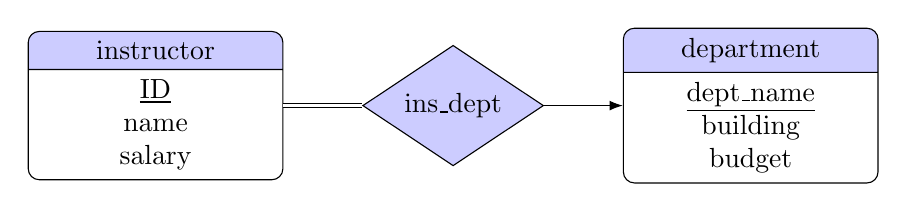
\begin{tikzpicture}[
			comment/.style={rectangle, draw=black, rounded corners,
					text centered, anchor=north, text=black, text width=3cm}, every second node part/.style={fill=white},]
		\node (instructor) [comment, rectangle split, rectangle split parts=2, rectangle split part fill={blue!20,white},]
		{
			instructor
			\nodepart{second} \underline{ID} \\ name \\ salary
		};

		\node (insdept) [fill=blue!20, draw, diamond, right=of instructor, aspect=1.5] {ins\_dept};

		\node (department) [comment, rectangle split, rectangle split parts=2, rectangle split part fill={blue!20,white}, right=of insdept] {
			department
			\nodepart{second} \underline{dept\_name} \\ building \\ budget
		};

		\draw [double, double distance=1.2pt] (instructor) -- (insdept);
		\draw [-Latex] (insdept) -- (department);
	\end{tikzpicture}

\end{frame}

{
% \usebackgroundtemplate{\transparent{0.3}{\begin{picture}
%     \includegraphics[height=0.7\paperheight]{cover}
% \end{picture}    
% }}
\usebackgroundtemplate{
	\tikz[overlay,remember picture]
	\node[opacity=0.3, at=(current page.south east),anchor=south east, yshift=2cm,xshift=4cm] {
		\includegraphics[height=0.6\paperheight]{cover}};
}
\begin{frame}
	\section{\textcolor{darkmidnightblue}{1. 好的设计}}
\end{frame}

}

\begin{frame}
	\frametitle{1.1 「大」的模式}
	\faIcon{lightbulb} 思考:为什么不用一个大的模式?即尽可能多地包含属性,比如\texttt{ins\_dept (ID, name, salary, dept\_name, building, budget)}

	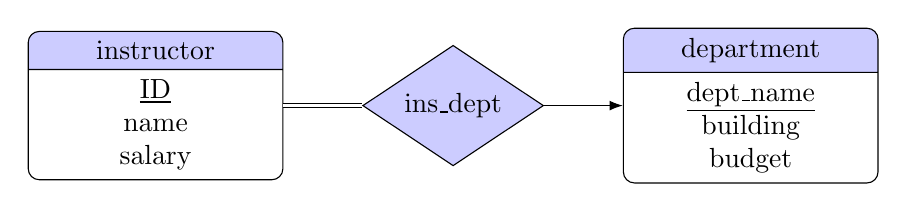
\begin{tikzpicture}[
			comment/.style={rectangle, draw=black, rounded corners,
					text centered, anchor=north, text=black, text width=3cm}, every second node part/.style={fill=white},]
		\node (instructor) [comment, rectangle split, rectangle split parts=2, rectangle split part fill={blue!20,white},]
		{
			instructor
			\nodepart{second} \underline{ID} \\ name \\ salary
		};

		\node (insdept) [fill=blue!20, draw, diamond, right=of instructor, aspect=1.5] {ins\_dept};

		\node (department) [comment, rectangle split, rectangle split parts=2, rectangle split part fill={blue!20,white}, right=of insdept] {
			department
			\nodepart{second} \underline{dept\_name} \\ building \\ budget
		};

		\draw [double, double distance=1.2pt] (instructor) -- (insdept);
		\draw [-Latex] (insdept) -- (department);
	\end{tikzpicture}

\end{frame}

\begin{frame}
	\frametitle{1.2 「小」的模式}
	合并后的「大」模式存在数据重复问题,那分解(decomposition)后得到「小」模式如何呢?

	\texttt{employee (ID, name, street, city, salary)}:

	\begin{itemize}
		\item employee1 (ID, name)
		\item employee2 (ID, street, city, salary)
	\end{itemize}

	或者
	\begin{itemize}
		\item employee1 (ID, name)
		\item employee2 (name, street, city, salary)
	\end{itemize}

\end{frame}

{\setbeamercolor{palette primary}{fg=black, bg=yellow}
\begin{frame}[standout]
	无损分解(lossless decomposition)是「好」的关系数据库设计的基础。

	\[\Pi_{R_1}(r) \Join  \Pi_{R_2}(r) = r\]
\end{frame}
}

\begin{frame}
	\frametitle{1.3 当我们说「好」,我们到底在说什么?}

	\faIcon{search} 查询资料,“师范大学”的英文怎么说?比如财大斜对面的“成都师范学院”。

	\pause
	\begin{exampleblock}{范式}
		我们说关系模式属于“好的形态/形式”(good form),表示它\alert{没有信息冗余}。这背后的理论依据就是检查是否符合\alert{范式}(normal form),并按需\alert{分解}。(课本p.179)
	\end{exampleblock}
\end{frame}

\begin{frame}
	\frametitle{规范化(normalization)}

	\begin{itemize}
		\item 检查关系模式是否属于“good form”,即检查其是否符合已知的范式。
		\item 如果它不属于“good form”,就将其分解。注意分解必须是无损分解。
	\end{itemize}

	\faIcon{map-marker} 最终目标是:\textbf{没有不必要的冗余,同时又能轻易地检索数据}。
\end{frame}

\begin{frame}
	\frametitle{1.4 第一范式(First Normal Norm)}

	查询资料,解释什么是关系模式的\alert{第一范式}(1NF)?

	\begin{table}
		\begin{tabular}{lll}
			\toprule
			stuID & Name  & Subject      \\
			\midrule
			101   & Alice & OS, Database \\
			102   & Bob   & Music        \\
			\bottomrule
		\end{tabular}
	\end{table}


	\begin{tikzpicture}
		\node[fill=yellow,blur shadow={shadow xshift=-0.5ex},
			text width=28em,anchor=south west,rounded corners]
		{第一范式(1NF)是对关系模式的基本要求,不满足第一范式(1NF)的数据库就不是关系数据库。};
	\end{tikzpicture}
\end{frame}

\begin{frame}
	\section{\textcolor{darkmidnightblue}{2. 利用函数依赖进行分解}}
	Functional dependencies
\end{frame}

\begin{frame}
	\frametitle{符号表示}
	\begin{itemize}
		\item \textbf{属性集}:使用希腊字母(如$\alpha$)
		\item \textbf{关系模式}:一般使用$r(R)$,其中$r$是关系名,$R$是属性列表。
		\item \textbf{超码}:当属性集是一个超码,使用$K$表示。我们可以是“K是R的一个超码”。
	\end{itemize}

	True or False: Given $r(R)$, a subset $K$ of $R$ is a superkey of $r(R)$ if, in any legal instance of $r(R)$, for all pairs $t_1$ and $t_2$ of tuples in the instance of $r$ if $t_1 \neq t_2$, then $t_1[K] \neq t_2[K]$.


\end{frame}

\begin{frame}
	\frametitle{2.1 函数依赖}
	\begin{exampleblock}{函数依赖}
		考虑一个关系模式$r(R)$,令$\alpha \subseteq R$且$\beta \subseteq R$。

		给定$r(R)$的一个实例,我们说这个实例满足(satisfy)\alert{函数依赖} $\alpha \rightarrow \beta$的条件是:对实例中的所有元组对$t_1$和$t_2$,若$t_1[\alpha] = t_2[\alpha]$,那么$t_1[\beta] = t_2[\beta]$。
	\end{exampleblock}

	如果在$r(R)$的每个合法实例都满足函数依赖$\alpha \rightarrow \beta$,则我们说该函数依赖在模式$r(R)$上成立(hold)。
\end{frame}

\begin{frame}
	\frametitle{练习}
	考虑大学数据库,指出下面的关系模式有哪些函数依赖?

	\texttt{ins\_dep (ID, name, salary, dept\_name, building, budget)
	}

\end{frame}

\begin{frame}
	\frametitle{平凡依赖}
	\begin{exampleblock}{平凡依赖}
		如果$\beta \subseteq \alpha$,那么函数依赖$\alpha \rightarrow \beta$就是\alert{平凡的}(trivial)。
	\end{exampleblock}

	比如,
	\begin{itemize}
		\item $ID \rightarrow ID$
		\item $ID, name \rightarrow name$
	\end{itemize}

	\textcolor{gray}{听君一席话 如听一席话;在非洲每60秒就有一分钟过去}
\end{frame}

\begin{frame}
	\frametitle{依赖闭包}
	函数依赖可以进行推断(运算),如从$A \rightarrow B$和$B \rightarrow C$可以推断$A \rightarrow C$。因此,函数依赖可以构成\alert{闭包}(closure)。我们用$F^+$表示集合$F$的闭包。

	\pause
	\begin{exampleblock}{依赖闭包和函数依赖}
		如果下面至少一个函数依赖属于$F^+$,那么$R_1$和$R_2$就构成了R的无损分解:

		\begin{itemize}
			\item $R_1 \cap R_2 \rightarrow R_1$
			\item $R_1 \cap R_2 \rightarrow R_2$
		\end{itemize}
	\end{exampleblock}

\end{frame}

\begin{frame}
	\frametitle{例子}
	请说明下面的分解是无损的:

	\texttt{ins\_dep (ID, name, salary, dept\_name, building, budget)
	}

	\begin{itemize}
		\item \texttt{instructor (ID, name, salary, dept\_name)    }
		\item \texttt{department (dept\_name, building, budget)}
	\end{itemize}


\end{frame}

\begin{frame}
	\frametitle{思考}
	假设我们将$r(R)$分解成$r_1(R_1)$和$r_2(R_2)$,并且$R_1 \cap R_2 \rightarrow R_1$。试分析:

	\begin{itemize}
		\item $r_1$的主码是什么?
		\item $r_2$的外码是什么?
	\end{itemize}


\end{frame}

\begin{frame}
	\frametitle{2.2 Boyce-Codd范式(BCNF)}
	我们能达到的较满意的范式之一就是\alert{Boyce-Codd范式}(BCNF)。\textbf{它消除所有基于函数依赖能够发现的冗余}。


	\begin{exampleblock}{BCNF}
		具有函数依赖集F的关系模式R属于BCNF的条件是,对$F^+$中所有形如$\alpha \rightarrow \beta$的函数依赖,下面至少一个成立:
		\begin{itemize}
			\item $\alpha \rightarrow \beta$是平凡的函数依赖
			\item $\alpha$是R的一个超码
		\end{itemize}

	\end{exampleblock}

\end{frame}

\begin{frame}

	\begin{exampleblock}{BCNF}
		具有函数依赖集F的关系模式R属于BCNF的条件是,对$F^+$中所有形如$\alpha \rightarrow \beta$的函数依赖,下面至少一个成立:
		\begin{itemize}
			\item $\alpha \rightarrow \beta$是平凡的函数依赖
			\item $\alpha$是R的一个超码
		\end{itemize}

	\end{exampleblock}

	\faIcon{lightbulb} 思考:\texttt{ins\_dep(ID, name, salary, dept\_name, building, budget)}是否满足BCNF?

\end{frame}

\begin{frame}
	\frametitle{练习1}
	考虑关系模式$(A, B, C, D, E)$,并有函数依赖$A \rightarrow B$和$BC \rightarrow D$。假设分解得到:

	\begin{itemize}
		\item (A, B)
		\item (A, C, D, E)
	\end{itemize}

	请问分解后的两个模式是否满足BCNF?


\end{frame}

\begin{frame}
	\frametitle{练习2}
	假设一个老师有多个地址,请对下面的关系模式进行分解,使其满足BCNF。

	\texttt{inst(ID, name, street, city)}

	\begin{table}
		\begin{tabular}{llll}
			\toprule
			ID    & name & street & city \\
			\midrule
			22222 & Bob  & 柳林     & 成都   \\
			22222 & Bob  & 光华     & 成都   \\
			33333 & Mike & 东川路    & 上海   \\
			\bottomrule
		\end{tabular}
	\end{table}


\end{frame}

\begin{frame}
	\frametitle{练习3}
	假设一个老师只能在一个学院,而一个学生可以在多个学院,请问下面的E-R图表示什么含义?关系模式\texttt{dept\_advisor}是否满足BCNF?

	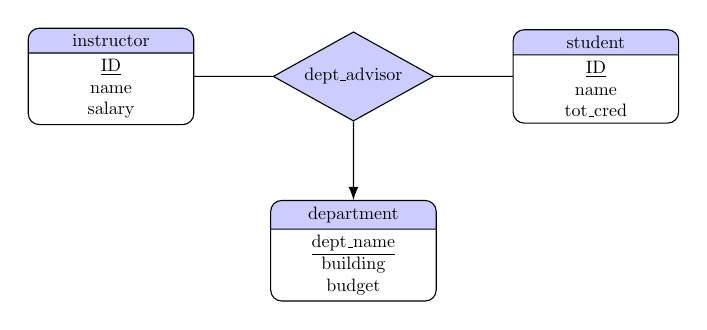
\begin{tikzpicture}[
			comment/.style={rectangle, draw=black, rounded corners,
					text centered, anchor=north, text=black, text width=3cm}, every second node part/.style={fill=white}, scale=0.65, every node/.style={scale=0.65}]
		\node (instructor) [comment, rectangle split, rectangle split parts=2, rectangle split part fill={blue!20,white}]
		{
			instructor
			\nodepart{second} \underline{ID} \\ name \\ salary
		};

		\node (deptadvisor) [fill=blue!20, draw, diamond, right=of instructor, aspect=1.8] {dept\_advisor};

		\node (student) [comment, rectangle split, rectangle split parts=2, rectangle split part fill={blue!20,white}, right=of deptadvisor] {
			student
			\nodepart{second} \underline{ID} \\ name \\ tot\_cred
		};

		\node (department) [comment, rectangle split, rectangle split parts=2, rectangle split part fill={blue!20,white}, below=of deptadvisor] {
			department
			\nodepart{second} \underline{dept\_name} \\ building \\ budget
		};

		\draw (instructor) -- (deptadvisor);
		\draw (deptadvisor) -- (student);
		\draw [Latex-] (department) -- (deptadvisor);
	\end{tikzpicture}

\end{frame}

\begin{frame}
	\frametitle{依赖保持}
	\texttt{dept\_advisor(s\_ID, i\_ID, dept\_name)},它包含的函数依赖:

	\begin{itemize}
		\item i\_ID $\rightarrow$ dept\_name
		\item s\_ID, dept\_name $\rightarrow$ i\_ID
	\end{itemize}

	分解后变成:

	\begin{itemize}
		\item \texttt{(s\_ID, i\_ID)}
		\item \texttt{(i\_ID, dept\_name)}
	\end{itemize}

	显然,BCNF会使得某些依赖丢失,必须通过Join才能得到,即它不是\alert{依赖保持}的(dependency preserving)。
\end{frame}


\begin{frame}
	\frametitle{2.3 第三范式(3NF)}
	\begin{exampleblock}{3NF}
		具有函数依赖集F的关系模式R属于3NF的条件是,对$F^+$中所有形如$\alpha \rightarrow \beta$的函数依赖,下面至少一个成立:
		\begin{itemize}
			\item $\alpha \rightarrow \beta$是平凡的函数依赖
			\item $\alpha$是R的一个超码
			\item $\beta - \alpha$的每个属性都属于R的某个候选码
		\end{itemize}
	\end{exampleblock}
	\faIcon{lightbulb} 试分析\texttt{dept\_advisor(s\_ID, i\_ID, dept\_name)}是否满足3NF?
\end{frame}

{\setbeamercolor{palette primary}{fg=black, bg=yellow}
\begin{frame}[standout]
	我们希望同时实现:

	\begin{itemize}
		\item BCNF
		\item 无损分解
		\item 依赖保持
	\end{itemize}

	{\small 第一点和第三点可能无法同时实现,这时可以在BCNF和3NF之间权衡。}
\end{frame}
}

\begin{frame}
	\frametitle{2.4 其他范式}
	\begin{itemize}
		\item 第二范式(2NF)只具备历史意义(课本p.182)。
		\item 4NF、5NF以及更高的范式很少被使用。对于一般数据库设计,\alert{都是在3NF和BCNF之间选择。}
	\end{itemize}


\end{frame}

\begin{frame}
	\frametitle{2.5 检查是否为BCNF}
	\begin{exampleblock}{检查非平凡依赖是否违反BCNF}
		对于每个非平凡依赖$\alpha \rightarrow \beta$,计算属性集$\alpha$的闭包,验证它是否包含所有R的属性;如果是,表明它就是超码。
	\end{exampleblock}
	这样考虑依赖$F$即可,而不需要考虑其闭包$F^+$。

	\pause
	\faIcon{pen} 例子:考虑关系模式\texttt{R = (A, B, C, D, E)},所包含函数依赖有:$A \rightarrow BC$,$CD \rightarrow E$,$B \rightarrow D$, $E \rightarrow A$。请问R是否符合BCNF?

\end{frame}

\begin{frame}
	\frametitle{2.6 BCNF分解算法}
	大致思路:找到R的某个非平凡函数依赖$\alpha \rightarrow \beta$,$\alpha$的闭包没有包含所有的属性,那么可以初步分解为:

	\begin{itemize}
		\item $R - \beta$
		\item $(\alpha, \beta)$
	\end{itemize}

\end{frame}

\begin{frame}
	\scalebox{.8}{
		\begin{algorithm}[H]
			\caption{BCNF decomposition}
			$result \gets \{R\}$ \\
			$done \gets false$ \\
			\While{not done}{
				\If{there is a schema $R_i$ that is not in BCNF}{
					let $\alpha \rightarrow \beta$ be a non-trivial FD that holds on $R_i$, such that $\alpha^+$ does not contain $R_i$ \\
					$result \gets (result - R_i) \cup (R_i - \beta) \cup (\alpha, \beta)$
				}\Else{
					$done \gets true$
				}
			}
		\end{algorithm}
	}
\end{frame}

\begin{frame}
	\frametitle{练习}

	考虑关系模式\texttt{R = (A, B, C, D, E)},所包含函数依赖有:$A \rightarrow BC$,$CD \rightarrow E$,$B \rightarrow D$, $E \rightarrow A$。请通过分解得到符合BCNF的模式。

\end{frame}

\begin{frame}
	\section{\textcolor{darkmidnightblue}{小结}}
	\begin{itemize}
		\item 模式分解
		\item 函数依赖
		\item BCNF, 3NF
	\end{itemize}
\end{frame}

\end{document}
